\documentclass[journal,12pt,twocolumn]{IEEEtran}
%
\usepackage{setspace}
\usepackage{gensymb}
\usepackage{xcolor}
\usepackage{caption}
%\usepackage{subcaption}
%\doublespacing
\usepackage{circuitikz}
\singlespacing

%\usepackage{graphicx}
%\usepackage{amssymb}
%\usepackage{relsize}
\usepackage[cmex10]{amsmath}
\usepackage{mathtools}
%\usepackage{amsthm}
%\interdisplaylinepenalty=2500
%\savesymbol{iint}
%\usepackage{txfonts}
%\restoresymbol{TXF}{iint}
%\usepackage{wasysym}
\usepackage{hyperref}
\usepackage{amsthm}
\usepackage{mathrsfs}
\usepackage{txfonts}
\usepackage{stfloats}
\usepackage{cite}
\usepackage{cases}
\usepackage{subfig}
%\usepackage{xtab}
\usepackage{longtable}
\usepackage{multirow}
%\usepackage{algorithm}
%\usepackage{algpseudocode}
%\usepackage{enumerate}
\usepackage{enumitem}
\usepackage{mathtools}
%\usepackage{iithtlc}
%\usepackage[framemethod=tikz]{mdframed}
\usepackage{listings}
\let\vec\mathbf


%\usepackage{stmaryrd}Showing results for how to add coordinates name in circuitikz
%Search instead for how to add cordinates name in circuitikz
%
%Search Results
%
%circuitikz - How to declare a custom coordinate - TeXhttps://tex.stackexchange.com › questions › how-to-dec...
%17-Mar-2019 · 1 answer
%You can define coordinates like this: \coordinate (c1) at ([xshift=-15mm]bothNegated.bin 1); \coordinate (c2) at ...
%circuitikz/tikz: x and y coordinates of anchors for adjusting ...
%10 Mar 2021
%TikZ: how to memorize current coordinate into a variable ...
%20 Feb 2019
%circuitikz - Tikz obtain node coordinates - TeX
%11 Dec 2014
%Transformer exact coordinates for circuit - TeX
%26 Apr 2020
%More results from tex.stackexchange.com


%\usepackage{wasysym}
%\newcounter{MYtempeqncnt}
\DeclareMathOperator*{\Res}{Res}
%\renewcommand{\baselinestretch}{2}
\renewcommand\thesection{\arabic{section}}
\renewcommand\thesubsection{\thesection.\arabic{subsection}}
\renewcommand\thesubsubsection{\thesubsection.\arabic{subsubsection}}

\renewcommand\thesectiondis{\arabic{section}}
\renewcommand\thesubsectiondis{\thesectiondis.\arabic{subsection}}
\renewcommand\thesubsubsectiondis{\thesubsectiondis.\arabic{subsubsection}}

%\renewcommand{\labelenumi}{\textbf{\theenumi}}
%\renewcommand{\theenumi}{P.\arabic{enumi}}

% correct bad hyphenation here
\hyphenation{op-tical net-works semi-conduc-tor}

\lstset{
language=Python,
frame=single, 
breaklines=true,
columns=fullflexible
}



\begin{document}
%

\theoremstyle{definition}
\newtheorem{theorem}{Theorem}[section]
\newtheorem{problem}{Problem}
\newtheorem{proposition}{Proposition}[section]
\newtheorem{lemma}{Lemma}[section]
\newtheorem{corollary}[theorem]{Corollary}
\newtheorem{example}{Example}[section]
\newtheorem{definition}{Definition}[section]
%\newtheorem{algorithm}{Algorithm}[section]
%\newtheorem{cor}{Corollary}
\newcommand{\BEQA}{\begin{eqnarray}}
\newcommand{\EEQA}{\end{eqnarray}}
\newcommand{\define}{\stackrel{\triangle}{=}}
\newcommand{\myvec}[1]{\ensuremath{\begin{pmatrix}#1\end{pmatrix}}}
\newcommand{\mydet}[1]{\ensuremath{\begin{vmatrix}#1\end{vmatrix}}}
\bibliographystyle{IEEEtran}
%\bibliographystyle{ieeetr}
\providecommand{\nCr}[2]{\,^{#1}C_{#2}} % nCr
\providecommand{\nPr}[2]{\,^{#1}P_{#2}} % nPr
\providecommand{\mbf}{\mathbf}
\providecommand{\pr}[1]{\ensuremath{\Pr\left(#1\right)}}
\providecommand{\qfunc}[1]{\ensuremath{Q\left(#1\right)}}
\providecommand{\sbrak}[1]{\ensuremath{{}\left[#1\right]}}
\providecommand{\lsbrak}[1]{\ensuremath{{}\left[#1\right.}}
\providecommand{\rsbrak}[1]{\ensuremath{{}\left.#1\right]}}
\providecommand{\brak}[1]{\ensuremath{\left(#1\right)}}
\providecommand{\lbrak}[1]{\ensuremath{\left(#1\right.}}
\providecommand{\rbrak}[1]{\ensuremath{\left.#1\right)}}
\providecommand{\cbrak}[1]{\ensuremath{\left\{#1\right\}}}
\providecommand{\lcbrak}[1]{\ensuremath{\left\{#1\right.}}
\providecommand{\rcbrak}[1]{\ensuremath{\left.#1\right\}}}
\theoremstyle{remark}
\newtheorem{rem}{Remark}
\newcommand{\sgn}{\mathop{\mathrm{sgn}}}
\providecommand{\abs}[1]{\left\vert#1\right\vert}
\providecommand{\res}[1]{\Res\displaylimits_{#1}} 
%\providecomand{\norm}[1]{\lVert#1\rVert}
\providecommand{\mtx}[1]{\mathbf{#1}}
\providecommand{\mean}[1]{E\left[ #1 \right]}
\providecommand{\fourier}{\overset{\mathcal{F}}{ \rightleftharpoons}}
\providecommand{\ztrans}{\overset{\mathcal{Z}}{ \rightleftharpoons}}
%\providecommand{\hilbert}{\overset{\mathcal{H}}{ \rightleftharpoons}}
\providecommand{\system}{\overset{\mathcal{H}}{ \longleftrightarrow}}
	%\newcommand{\solution}[2]{\textbf{Solution:}{#1}}
\newcommand{\solution}{\noindent \textbf{Solution: }}
\providecommand{\dec}[2]{\ensuremath{\overset{#1}{\underset{#2}{\gtrless}}}}
\numberwithin{equation}{section}
%\numberwithin{equation}{subsection}
%\numberwithin{problem}{subsection}
%\numberwithin{definition}{subsection}
\makeatletter
\@addtoreset{figure}{problem}
\makeatother
\let\StandardTheFigure\thefigure
%\renewcommand{\thefigure}{\theproblem.\arabic{figure}}
\renewcommand{\thefigure}{\theproblem}
%\numberwithin{figure}{subsection}
\def\putbox#1#2#3{\makebox[0in][l]{\makebox[#1][l]{}\raisebox{\baselineskip}[0in][0in]{\raisebox{#2}[0in][0in]{#3}}}}
     \def\rightbox#1{\makebox[0in][r]{#1}}
     \def\centbox#1{\makebox[0in]{#1}}
     \def\topbox#1{\raisebox{-\baselineskip}[0in][0in]{#1}}
     \def\midbox#1{\raisebox{-0.5\baselineskip}[0in][0in]{#1}}
\vspace{3cm}
\title{ 
%\logo{
%}
Circuits and Transforms
%	\logo{Octave for Math Computing }
}
%\title{
%	\logo{Matrix Analysis through Octave}{\begin{center}\includegraphics[scale=.24]{tlc}\end{center}}{}{HAMDSP}
%}
% paper title
% can use linebreaks \\ within to get better formatting as desired
%\title{Matrix Analysis through Octave}
%
%
% author names and IEEE memberships
% note positions of commas and nonbreaking spaces ( ~ ) LaTeX will not break
% a structure at a ~ so this keeps an author's name from being broken across
% two lines.
% use \thanks{} to gain access to the first footnote area
% a separate \thanks must be used for each paragraph as LaTeX2e's \thanks
% was not built to handle multiple paragraphs
%
\author{ Himanshu Kumar Gupta%<-this  stops a space
% <-this % stops a space
%\thanks{J. Doe and J. Doe are with Anonymous University.}% <-this % stops a space
%\thanks{Manuscript received April 19, 2005; revised January 11, 2007.}}
}
% note the % following the last \IEEEmembership and also \thanks - 
% these prevent an unwanted space from occurring between the last author name
% and the end of the author line. i.e., if you had this:
% 
% \author{....lastname \thanks{...} \thanks{...} }
%                     ^------------^------------^----Do not want these spaces!
%
% a space would be appended to the last name and could cause every name on that
% line to be shifted left slightly. This is one of those "LaTeX things". For
% instance, "\textbf{A} \textbf{B}" will typeset as "A B" not "AB". To get
% "AB" then you have to do: "\textbf{A}\textbf{B}"
% \thanks is no different in this regard, so shield the last } of each \thanks
% that ends a line with a % and do not let a space in before the next \thanks.
% Spaces after \IEEEmembership other than the last one are OK (and needed) as
% you are supposed to have spaces between the names. For what it is worth,
% this is a minor point as most people would not even notice if the said evil
% space somehow managed to creep in.
% The paper headers
%\markboth{Journal of \LaTeX\ Class Files,~Vol.~6, No.~1, January~2007}%
%{Shell \MakeLowercase{\textit{et al.}}: Bare Demo of IEEEtran.cls for Journals}
% The only time the second header will appear is for the odd numbered pages
% after the title page when using the twoside option.
% 
% *** Note that you probably will NOT want to include the author's ***
% *** name in the headers of peer review papers.                   ***
% You can use \ifCLASSOPTIONpeerreview for conditional compilation here if
% you desire.
% If you want to put a publisher's ID mark on the page you can do it like
% this:
%\IEEEpubid{0000--0000/00\$00.00~\copyright~2007 IEEE}
% Remember, if you use this you must call \IEEEpubidadjcol in the second
% column for its text to clear the IEEEpubid mark.
% make the title area
\maketitle
%\newpage
\tableofcontents
%\renewcommand{\thefigure}{\thesection.\theenumi}
%\renewcommand{\thetable}{\thesection.\theenumi}
\renewcommand{\thefigure}{\theenumi}
\renewcommand{\thetable}{\theenumi}
%\renewcommand{\theequation}{\thesection}
\bigskip
\begin{abstract}
This manual provides a simple introduction to Transforms
\end{abstract}
%% Copyright (C) 2020 Saurabh Joshi
%% 
%\let\negmedspace\undefined
%\let\negthickspace\undefined
%\documentclass[journal,12pt,onecolumn]{IEEEtran}
%%\documentclass[journal,12pt,twocolumn]{IEEEtran}
%%
%\usepackage{setspace}
%\usepackage{gensymb}
%%\doublespacing
%\singlespacing
%
%%\usepackage{graphicx}
%%\usepackage{amssymb}
%%\usepackage{relsize}
%\usepackage[cmex10]{amsmath}
%%\usepackage{amsthm}
%%\interdisplaylinepenalty=2500
%%\savesymbol{iint}
%%\usepackage{txfonts}
%%\restoresymbol{TXF}{iint}
%%\usepackage{wasysym}
%\usepackage{amsthm}
%\usepackage{mathrsfs}
%\usepackage{txfonts}
%\usepackage{stfloats}
%\usepackage{cite}
%\usepackage{cases}
%\usepackage{subfig}
%%\usepackage{xtab}
%\usepackage{longtable}
%\usepackage{multirow}
%%\usepackage{algorithm}
%%\usepackage{algpseudocode}
%\usepackage{enumitem}
%\usepackage{mathtools}
%\usepackage{tikz}
%\usetikzlibrary{shapes,arrows,positioning}
%\usepackage{verbatim}
%\usepackage{hyperref}
%%\usepackage{stmaryrd}
%\usepackage{tkz-euclide} % loads  TikZ and tkz-base
%%\usetkzobj{all}
%\usepackage{listings}
%    \usepackage{color}                                            %%
%    \usepackage{array}                                            %%
%    \usepackage{longtable}                                        %%
%    \usepackage{calc}                                             %%
%    \usepackage{multirow}                                         %%
%    \usepackage{hhline}                                           %%
%    \usepackage{ifthen}                                           %%
%  %optionally (for landscape tables embedded in another document): %%
%    \usepackage{lscape}     
%\usepackage{multicol}
%\usepackage{chngcntr}
%\usepackage{iftex}
%%\usepackage[latin9]{inputenc}
%\usepackage{geometry}
%%\geometry{verbose,tmargin=2cm,bmargin=3cm,lmargin=1.8cm,rmargin=1.5cm,headheight=2cm,headsep=2cm,footskip=3cm}
%\usepackage{array}
%\newcolumntype{L}[1]{>{\raggedright\let\newline\\\arraybackslash\hspace{0pt}}m{#1}}
%\newcolumntype{C}[1]{>{\centering\let\newline\\\arraybackslash\hspace{0pt}}m{#1}}
%\newcolumntype{R}[1]{>{\raggedleft\let\newline\\\arraybackslash\hspace{0pt}}m{#1}}
% \usepackage{float}
%%\usepackage{graphicx}
%%\usepackage{setspace}
%%\usepackage{parskip}
%
%\def \hsp {\hspace{3mm}}
%
%\makeatletter
%
%\providecommand{\tabularnewline}{\\}
%
%
%\makeatother
%\ifxetex
%\usepackage[T1]{fontenc}
%\usepackage{fontspec}
%%\setmainfont[ Path = fonts/]{Sanskrit_2003.ttf}
%\newfontfamily\nakulafont[Script=Devanagari,AutoFakeBold=2,Path = fonts/]{Nakula}
%%\newfontfamily\liberationfont{Liberation Sans Narrow}
%%\newfontfamily\liberationsansfont{Liberation Sans}
%\fi
%\usepackage{tikz}
%\usepackage{xcolor}
%%\usepackage{enumerate}
%
%%\usepackage{wasysym}
%%\newcounter{MYtempeqncnt}
%\DeclareMathOperator*{\Res}{Res}
%%\renewcommand{\baselinestretch}{2}
%\renewcommand\thesection{\arabic{section}}
%\renewcommand\thesubsection{\thesection.\arabic{subsection}}
%\renewcommand\thesubsubsection{\thesubsection.\arabic{subsubsection}}
%
%\renewcommand\thesectiondis{\arabic{section}}
%\renewcommand\thesubsectiondis{\thesectiondis.\arabic{subsection}}
%\renewcommand\thesubsubsectiondis{\thesubsectiondis.\arabic{subsubsection}}
%
%% correct bad hyphenation here
%\hyphenation{op-tical net-works semi-conduc-tor}
%\def\inputGnumericTable{}                                 %%
%
%\lstset{
%language=tex,
%frame=single, 
%breaklines=true
%}
%
%%\begin{document}
%%
%
%
%\newtheorem{theorem}{Theorem}[section]
%\newtheorem{problem}{Problem}
%\newtheorem{proposition}{Proposition}[section]
%\newtheorem{lemma}{Lemma}[section]
%\newtheorem{corollary}[theorem]{Corolhow to scrool down in vimlary}
%\newtheorem{example}{Example}[section]
%\newtheorem{definition}[problem]{Definition}
%%\newtheorem{thm}{Theorem}[section] 
%%\newtheorem{defn}[thm]{Definition}
%%\newtheorem{algorithm}{Algorithm}[section]
%%\newtheorem{cor}{Corollary}
%\newcommand{\BEQA}{\begin{eqnarray}}
%\newcommand{\EEQA}{\end{eqnarray}}
%\newcommand{\define}{\stackrel{\triangle}{=}}
%
%\bibliographystyle{IEEEtran}
%%\bibliographystyle{ieeetr}
%
%
%\providecommand{\mbf}{\mathbf}
%\providecommand{\pr}[1]{\ensuremath{\Pr\left(#1\right)}}
%\providecommand{\qfunc}[1]{\ensuremath{Q\left(#1\right)}}
%\providecommand{\sbrak}[1]{\ensuremath{{}\left[#1\right]}}
%\providecommand{\lsbrak}[1]{\ensuremath{{}\left[#1\right.}}
%\providecommand{\rsbrak}[1]{\ensuremath{{}\left.#1\right]}}
%\providecommand{\brak}[1]{\ensuremath{\left(#1\right)}}
%\providecommand{\lbrak}[1]{\ensuremath{\left(#1\right.}}
%\providecommand{\rbrak}[1]{\ensuremath{\left.#1\right)}}
%\providecommand{\cbrak}[1]{\ensuremath{\left\{#1\right\}}}
%\providecommand{\lcbrak}[1]{\ensuremath{\left\{#1\right.}}
%\providecommand{\rcbrak}[1]{\ensuremath{\left.#1\right\}}}
%\theoremstyle{remark}
%\newtheorem{rem}{Remark}
%\newcommand{\sgn}{\mathop{\mathrm{sgn}}}
%\providecommand{\abs}[1]{\left\vert#1\right\vert}
%\providecommand{\res}[1]{\Res\displaylimits_{#1}} 
%\providecommand{\norm}[1]{\left\lVert#1\right\rVert}
%%\providecommand{\norm}[1]{\lVert#1\rVert}
%\providecommand{\mtx}[1]{\mathbf{#1}}
%\providecommand{\mean}[1]{E\left[ #1 \right]}
%\providecommand{\fourier}{\overset{\mathcal{F}}{ \rightleftharpoons}}
%%\providecommand{\hilbert}{\overset{\mathcal{H}}{ \rightleftharpoons}}
%%\providecommand{\system}{\overset{\mathcal{H}}{ \longleftrightarrow}}
%\providecommand{\system}[1]{\overset{\mathcal{#1}}{ \longleftrightarrow}}
%\newcommand{\sinc}{\,\text{sinc}\,}
%\newcommand{\rect}{\,\text{rect}\,}
%	%\newcommand{\solution}[2]{\textbf{Solution:}{#1}}
%\newcommand{\solution}{\noindent \textbf{Solution: }}
%\newcommand{\cosec}{\,\text{cosec}\,}
%\providecommand{\dec}[2]{\ensuremath{\overset{#1}{\underset{#2}{\gtrless}}}}
%\newcommand{\myvec}[1]{\ensuremath{\begin{pmatrix}#1\end{pmatrix}}}
%\newcommand{\mydet}[1]{\ensuremath{\begin{vmatrix}#1\end{vmatrix}}}
%\newcommand*{\permcomb}[4][0mu]{{{}^{#3}\mkern#1#2_{#4}}}
%\newcommand*{\perm}[1][-3mu]{\permcomb[#1]{P}}
%\newcommand*{\comb}[1][-1mu]{\permcomb[#1]{C}}
%%\numberwithin{equation}{section}
%\numberwithin{equation}{section}
%%\numberwithin{problem}{section}
%%\numberwithin{definition}{section}
%\makeatletter
%\@addtoreset{figure}{problem}
%\makeatother
%
%\let\StandardTheFigure\thefigure
%\let\vec\mathbf
%%\renewcommand{\thefigure}{\theproblem.\arabic{figure}}
%\renewcommand{\thefigure}{\theproblem}
%%\setlist[enumerate,1]{before=\renewcommand\theequation{\theenumi.\arabic{equation}}
%%\counterwithin{equation}{enumi}
%
%
%%\renewcommand{\theequation}{\arabic{subsection}.\arabic{equation}}
%
%\vspace{3cm}
%
%
%%\usepackage{babel}
%\begin{document}
%
%\begin{tabular}{L{6cm} C{2cm} R{5cm} }
%
%	\definecolor{circleorange}{rgb}{1,0.17,0.08}
%\definecolor{darkorange}{rgb}{1,0.27,0.1}
%\definecolor{orange2}{rgb}{1,0.5,0.15}
%\definecolor{orange3}{rgb}{1,0.65,0.25}
%\definecolor{yellow1}{rgb}{0.95,0.77,0.2}
%%\begin{tikzpicture}[scale=0.2,every node/.style={transform shape}]
%\begin{tikzpicture}[scale=0.1,every node/.style={transform shape}]
%\draw [fill=circleorange,circleorange] (5,10) circle (1.15); 
%\fill [darkorange] (5.06,8) -- (5.06,2) -- (7.3,1.2) -- (7.3,8.8) -- (5.06,8);
%\fill [darkorange] (4.94,8) -- (4.94,2) -- (2.7,1.2) -- (2.7,8.8) -- (4.94,8);
%\fill [orange2]    (7.4,8.4) -- (7.4,1.6) -- (8.2,1.2) -- (8.2,8.8) -- (7.4,8.4);
%\fill [orange2]    (2.6,8.4) -- (2.6,1.6) -- (1.8,1.2) -- (1.8,8.8) -- (2.6,8.4);
%\fill [orange3]    (8.3,8.4) -- (8.3,1.6) -- (9.0,1.2) -- (9.0,8.8) -- (8.3,8.4);
%\fill [orange3]    (1.7,8.4) -- (1.7,1.6) -- (1.0,1.2) -- (1.0,8.8) -- (1.7,8.4);
%\fill [yellow1]    (9.1,8.4) -- (9.1,1.6) -- (9.7,1.2) -- (9.7,8.8) -- (9.1,8.4);
%\fill [yellow1]    (0.9,8.4) -- (0.9,1.6) -- (0.3,1.2) -- (0.3,8.8) -- (0.9,8.4);
%\ifxetex
%\node [scale=2.1] at (5,-0.1)  {   {\bf {\nakulafont  भारतीय प्रौद्योगिकी संस्थान हैदराबाद }} };
%\node [scale=1.8] at (5,-1.2) {   {\bf { Indian Institute of Technology Hyderabad}} };
%%\node [scale=1.8] at (5,-1.2) {   {\bf {\liberationsansfont Indian Institute of Technology Hyderabad}} };
%\fi
%\end{tikzpicture}
%% \includegraphics[scale=0.05]{logo_iith} \newline
%
%& Quiz  13
%	&
%EE3900	
%\end{tabular}
%
%
%\vspace{-6mm}
%\begin{center}
%%\includegraphics[scale=0.95]{Yellow-Line}
%\begin{tikzpicture}
%\definecolor{yellow1}{rgb}{0.95,0.77,0.2}
%\draw[line width=0.75mm, yellow1] (0,0) -- (\textwidth,0);
%\end{tikzpicture}
%\par\end{center}
 \section{Definitions}
\begin{enumerate}[label=\arabic*.,ref=\thesection.\theenumi]
\numberwithin{equation}{section}
\numberwithin{figure}{section}
\item The unit step function is 
\begin{align}
u(t) =
\begin{cases}
1 & t > 0
\\
	\frac{1}{2} & t = 0
\\
0 & t < 0
\end{cases}
\end{align}
\item The Laplace transform of $g(t)$ is defined as 
\begin{align}
	G(s) = \int_{-\infty}^{\infty} g(t) e^{-st}\, dt
\end{align}
 \end{enumerate}
 \section{Laplace Transform}
\begin{enumerate}[label=\arabic*.,ref=\thesection.\theenumi]
\numberwithin{equation}{section}
\item In the circuit, the switch S is connected to position P for a long time so that the charge on the capacitor
	becomes $q_1 \, \mu C$. Then S is switched to position Q.  After a long time, the charge on the capacitor is
		$q_2 \, \mu C$.
		\begin{figure}[!ht]
			\centering
			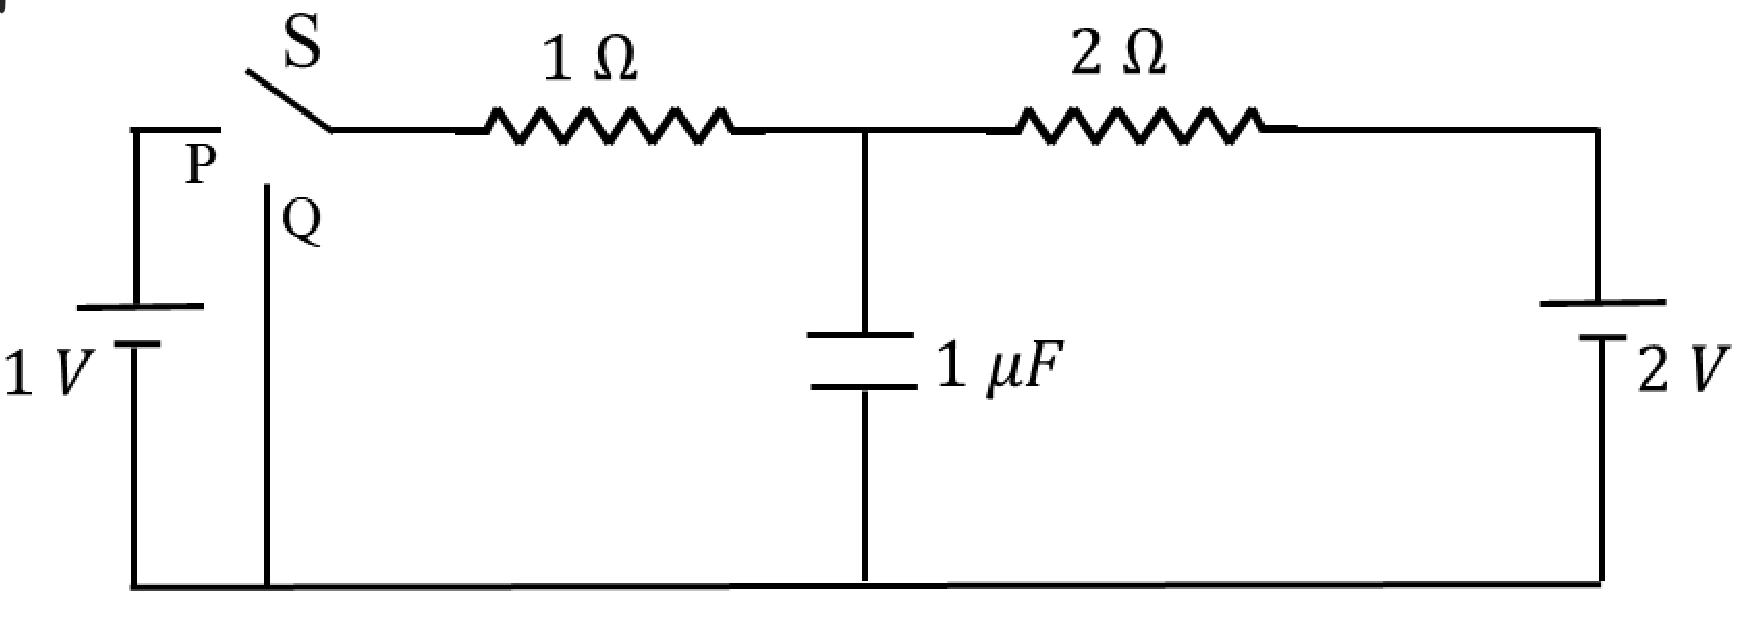
\includegraphics[width=\columnwidth]{figs/ckt.jpg}
			\caption{}
			\label{fig:ckt}
\end{figure}
\item Draw the circuit using latex-tikz.
	\solution See fig. \ref{crct:2.2}
\begin{figure}[!ht]
			\begin{circuitikz} \draw
			(.5,3)node[anchor=north east]{P}--(0,3) to[battery1,l_=1V] (0,0)
			(0,3)--(.5,3)
			(1,0)--(1,2.5)node[anchor=north west]{Q}
			(0,0)--(6,0)
			(1,3)to[R=$1\Omega$](3,3)to[R=$2\Omega$](6,3)
			(1,3)--(.6,3.4)node[anchor=south west]{S}
			(6,3) to[battery1,l=2V] (6,0)
			(3,0) to[C,l_=$\mu F$] (3,3);
		\end{circuitikz}

	\centering
	\caption{Given Circuit}
	\label{crct:2.2}
\end{figure}
\item Find $q_1$.
	\solution
		On connecting S to P for a long time capacitor get fully charged behave like disconnected wire. So, circuit will look like \ref{crct:2.3}
\begin{figure}[!ht]
	\begin{circuitikz} \draw
			(.5,3)--(0,3) to[battery1,l_=1V] (0,0)
			(0,0)--(3,0)node[anchor=south]{M}--(6,0)
			(0,3)to[R=$1\Omega$](3,3)node[anchor=north]{N} to[R=$2\Omega$](6,3)
			(6,3) to[battery1,l=2V] (6,0);
		\end{circuitikz}

	\centering
	\caption{circuit when conected to P for long time}
	\label{crct:2.3}
\end{figure}
		On applying KVL on circuit in fig. \ref{crct:2.3} we get current as,
		\begin{align}
			i=1/3	
		\end{align}
in counter-clockwise direction
So, PD across the capacitor i.e. across M and N is given by,
		\begin{align}
			v_{C_0}&=1+\frac{1}{3}\times 1\\
			&=\frac{4}{3}
		\end{align}
		So, charge on capacitor will be
		\begin{align}
			q_1&=v_{C_0}C_0\\
			&=\frac{4}{3}\mu C
		\end{align}
			
	\item Show that the Laplace transform of $u(t)$ is $\frac{1}{s}$ and find the ROC.
		\solution Laplace of u(t) is given by
		\begin{align}
			U(t)&=\int_{-\infty}^{\infty} u(t) e^{-st}\, dt\\
			&=\int_{0}^{\infty} e^{-st}\, dt\\
			&=\frac{e^{-st}}{-s}\bigg]_0^\infty\\
			&=\frac{1}{s}
		\end{align}
Since $e^{-st}$ is defined at $t\to \infty$ only for $s>0$
So, ROC will be $s>0$
	\item Show that 
		\begin{align}
			e^{-at}u(t) \system{L} \frac{1}{s+a}, \quad a > 0
		\end{align}
		and find the ROC.
		\solution
		\begin{align}
			\mathcal{L}\sbrak{e^{-at}u(t)}&=\int_{-\infty}^{\infty} e^{-at}u(t) e^{-st}\, dt\\
			&=\int_{-\infty}^{\infty} e^{-at}u(t) e^{-st}\, dt\\
			&=\int_{0}^{\infty} e^{-(a+s)t} \, dt\\
			&=\frac{e^{-(s+a)t}}{-(s+a)}\bigg]_0^\infty\\
			&=\frac{1}{s+a}
		\end{align}
		Since $e^{-(s+a)t}$ is defined at $t\to \infty$ only for $s>-a$
		So, ROC will be $s>-a$
	\item Now consider the following resistive circuit transformed from 
			Fig. \ref{fig:ckt}
		\begin{figure}[!ht]
			\centering
			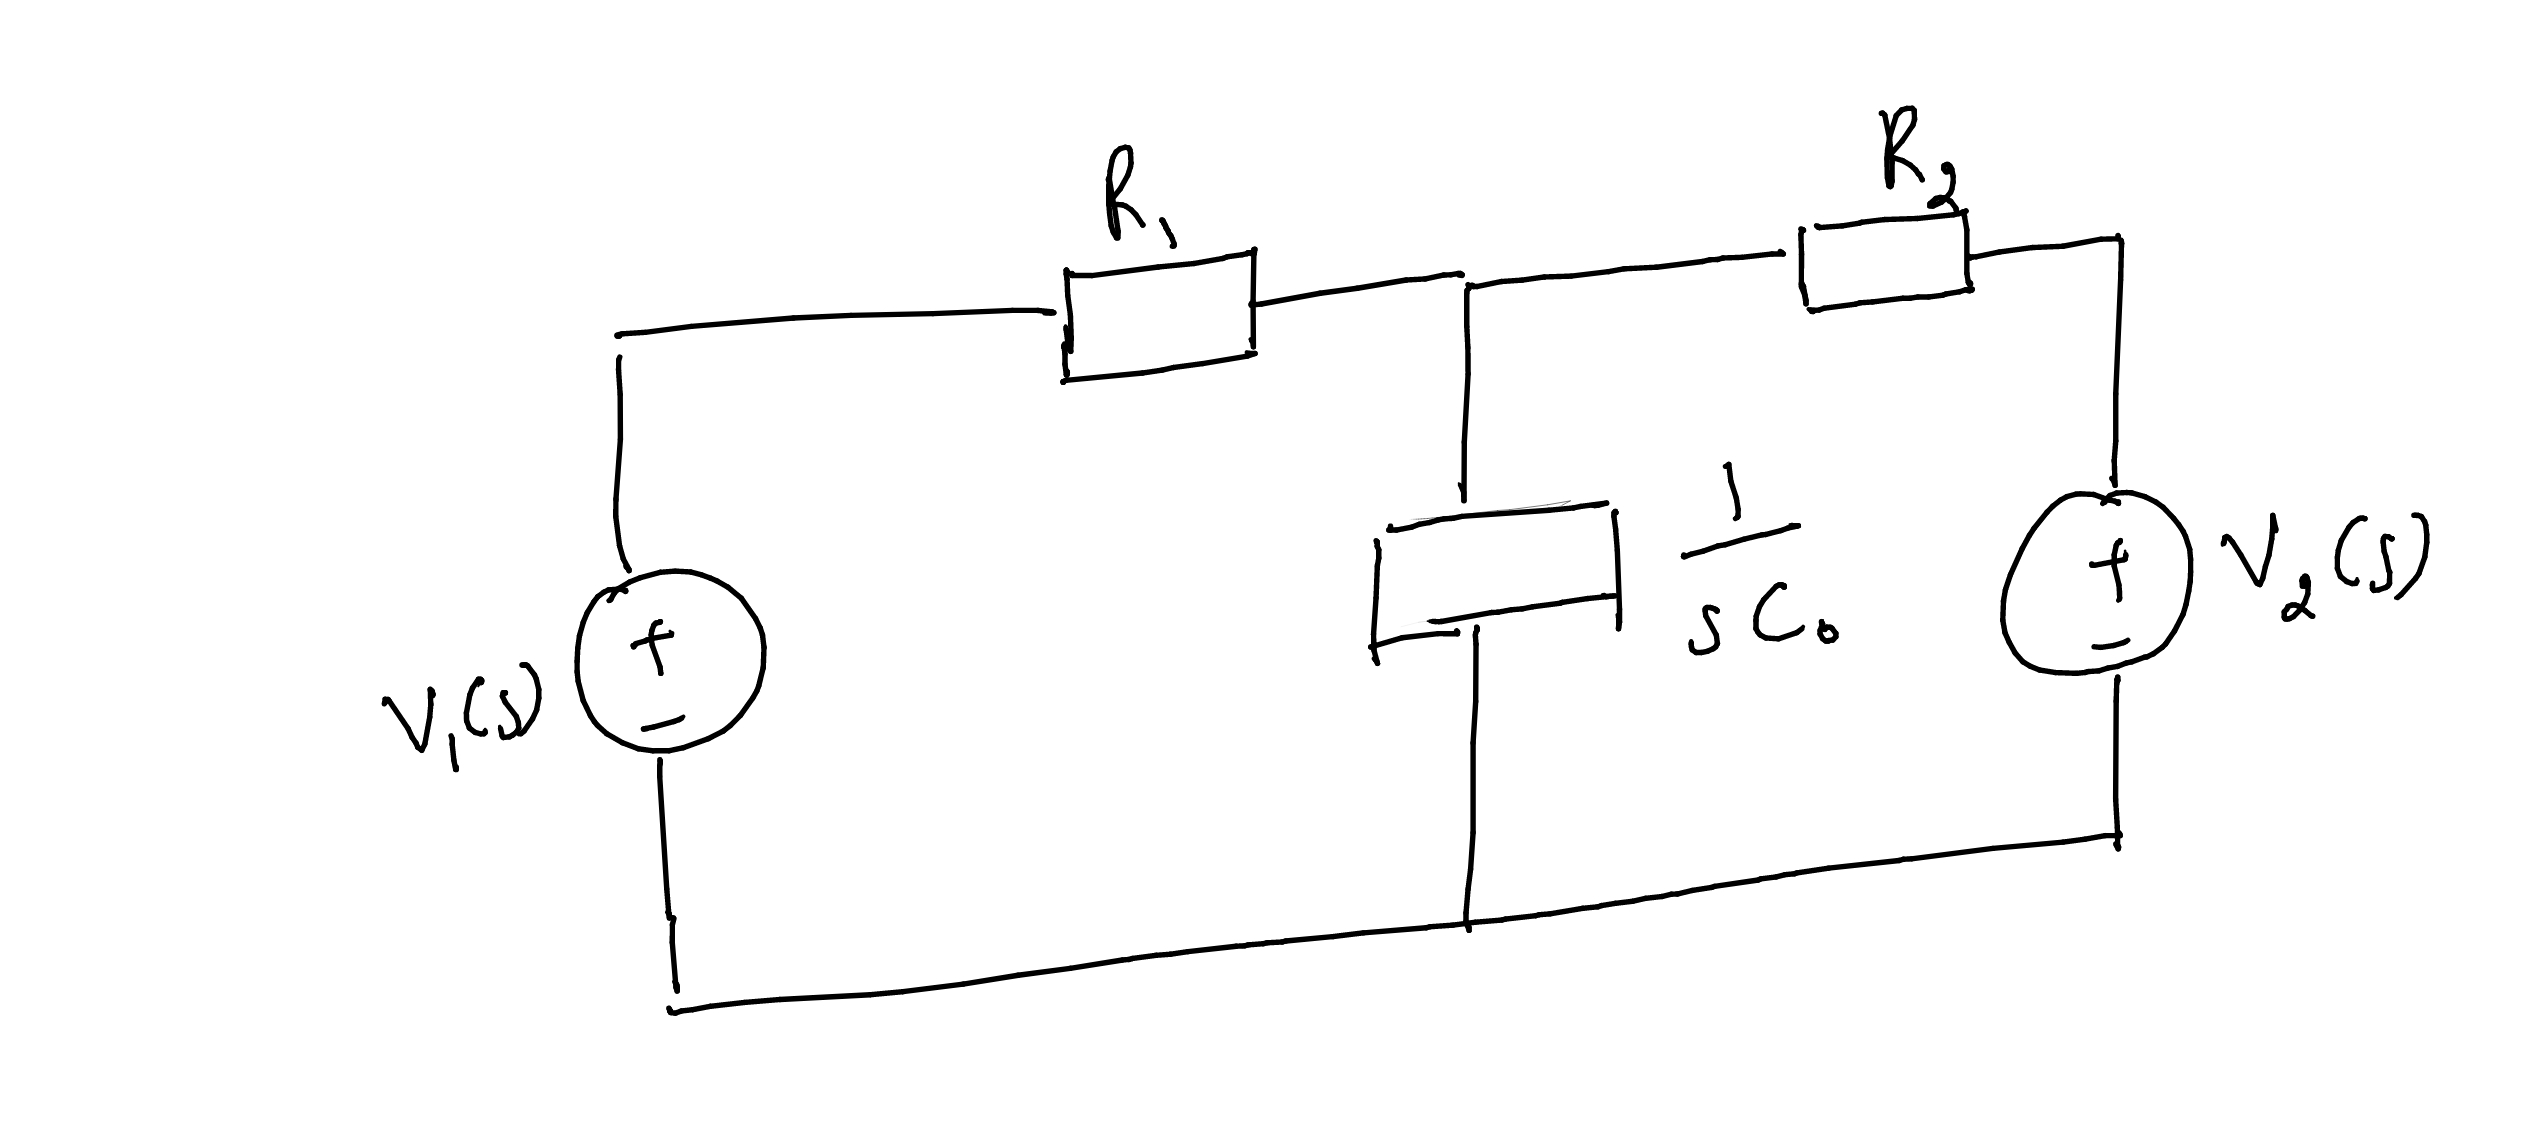
\includegraphics[width=\columnwidth]{figs/lap-ckt.jpg}
			\caption{hbhb}
			\label{fig:lap-ckt}
\end{figure}
		where 
		\begin{align}
			u(t) \system{L} V_1(s)
			\\
			2u(t) \system{L} V_2(s)
		\end{align}
		Find the voltage across the capacitor $V_{C_0}(s)$.
		
		\solution
\begin{figure}[!ht]
	\begin{circuitikz} \draw
			(.5,3)--(0,3) to[battery1,l_=1V] (0,0)
			(0,0)--(3,0)node[anchor=north east]{R}--(6,0)
			(0,3)to[generic=$1\Omega$](3,3)node[anchor=south east]{S}to[generic=$2\Omega$](6,3)
			(6,3) to[battery1,l=2V] (6,0)
			(3,0) to[generic,l_=$\frac{1}{sC_0}$] (3,3);
		\end{circuitikz}

	\centering
	\caption{s-domain resistive circuit}
	\label{crct:2.6}
\end{figure}
		from above 2 equations we can conclude that $V_1(s)=\frac{1}{s}$ and $V_2(s)=\frac{2}{s}$
		Now, let voltage at point R is 0. Applying KCL at point S i.e. junction of 3 resistors we get
		\begin{align}
			\frac{V_S(s)-0}{1/sC_0}+&\frac{V_S(s)-1/s}{1}+\frac{V_S(s)-2/s}{2}=0\\
		\implies	V_S(s)&=\frac{4}{s(3+2s)}
		\end{align}
		Now, the voltage across capacitor is given by
		\begin{align}
			V_{C_0}(s)&=V_S-V_R\\
			&=\frac{4}{s(3+2s)}
		\end{align}
	\item Find $v_{C_0}(t)$.  Plot using python.
		\solution $v_{C_0}(t)$ is given by
			\begin{align}
				v_{C_0}(t)&=\mathcal{L}^{-1}\sbrak{V_{C_0}(s)}\\
				&=\mathcal{L}^{-1}\sbrak{\frac{4}{s(3+2s)}}\\
				&=\frac{4}{3}\brak{\mathcal{L}^{-1}\sbrak{\frac{1}{s}}-\mathcal{L}^{-1}\sbrak{\frac{1}{s+3/2}}}\\
				&=\frac{4}{3}\brak{1-e^{-\frac{3}{2}}}u(t)
				\end{align}
Run below python code to get fig. \ref{fig:v_t_1} which is of $v_{C_0}(t)$
\begin{figure}[!ht]
	\centering
	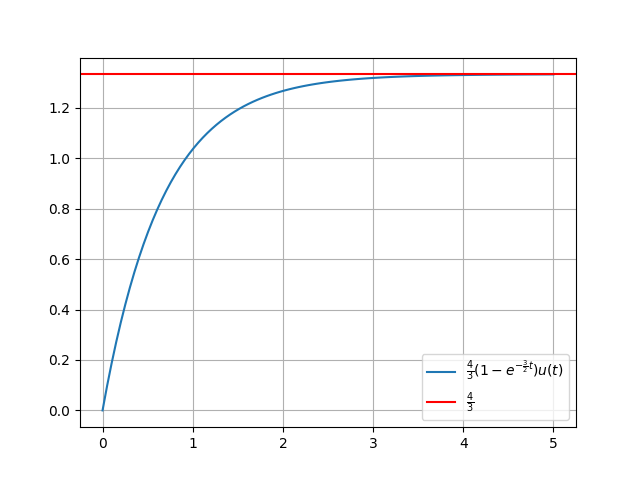
\includegraphics[width=\columnwidth]{./ques_2/v_t_1.png}
\label{fig:v_t_1}
\caption{$v_{C_0}(t)$ wrt t}	
\end{figure}
	\item Verify your result using ngspice.
		\solution Run the below ngspice code to get data and then use given python file to plot fig. \ref{fig:2.8}
		In fig. \ref{fig:2.8}, we can see that both results are coinciding. So, our answer is correct
\begin{lstlisting}
https://github.com/himanshukumargupta11012/EE3900_assignments/blob/main/cktsig/ques_2/2.8.cir
https://github.com/himanshukumargupta11012/EE3900_assignments/blob/main/cktsig/ques_2/2.8.py
		\end{lstlisting}
\begin{figure}[!ht]
	\centering
	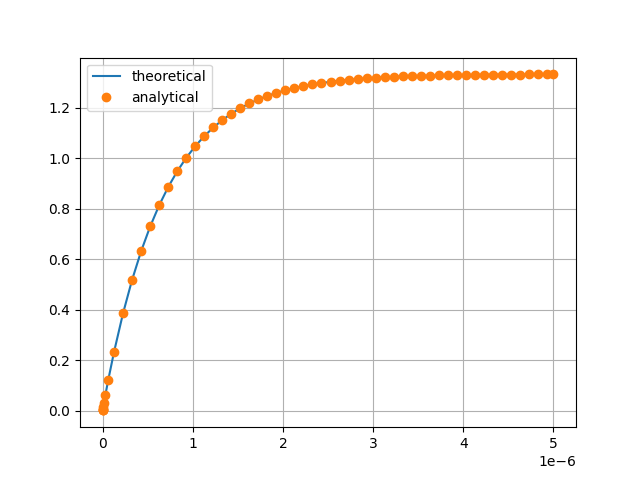
\includegraphics[width=\columnwidth]{./ques_2/2.8.png}
	\caption{theoretical v/s analytical}	
	\label{fig:2.8}
\end{figure}
	\item Obtain Fig. 
			\ref{fig:lap-ckt}
			using the equivalent differential equation.
			\solution Using KCL at the junction of resistors and capacitor, we get
			\begin{align}
				\frac{v_{C}(t)-v_1(t)}{R_1}+\frac{v_{C}(t)-v_{2}(t)}{R_2}+\frac{dq(t)}{dt}=0\\
			\end{align}
where $q(t)$ is charge on capacitor
Taking laplace both sides, we get
\begin{align}
	\frac{V_{C}(s)-0}{R_1}+\frac{V_{C}(s)-V_{2}(s)}{R_2}+sQ(s)-q(0)=0\\
	\frac{V_{C}(s)-0}{R_1}+\frac{V_{C}(s)-V_{2}(s)}{R_2}+sC_0\frac{Q(s)}{C_0}-0=0\\
	\frac{V_{C}(s)-0}{R_1}+\frac{V_{C}(s)-V_{2}(s)}{R_2}+sC_0V_{C}=0\\
	\frac{V_{C}(s)-0}{R_1}+\frac{V_{C}(s)-V_{2}(s)}{R_2}+\frac{V_{C}(s)}{\frac{1}{sC_0}}=0\\
\end{align}
The above equation is same as Fig. \ref{fig:lap-ckt} 
\end{enumerate}
 \section{Initial Conditions}
\begin{enumerate}[label=\arabic*.,ref=\thesection.\theenumi]
\numberwithin{equation}{section}
\item Find $q_2$ in Fig. 
			\ref{fig:ckt}.
			\solution
			Since S is connected to Q for a long time so capacitor get fully charged and behave as a disconnected wire. So, the circuit will look like this
			
\begin{figure}[!ht]
	\begin{circuitikz} \draw
			(.5,3)--(0,3)--(0,0)
			(0,0)--(3,0)--(6,0)
			(0,3)to[R=$1\Omega$](3,3)to[R=$2\Omega$](6,3)
			(6,3) to[battery1,l=2V] (6,0);
		\end{circuitikz}

	\centering
	\caption{when connected to Q for long time}
	\label{crct:3.1}
\end{figure}
		So, current in the circuit is given by
		\begin{align}
			i=\frac{2}{3}A
		\end{align}
		in counter-clockwise direction
		So, voltage across capacitor is given by
		\begin{align}
			v_{C_0}=\frac{2}{3}\times1=\frac{2}{3}
		\end{align}
		So, $q_2$ will be
		\begin{align}
			q_2&=V_{C_0}C_0\\
			&=\frac{2}{3}\mu C
		\end{align}
\item Draw the equivalent $s$-domain resistive circuit when S is switched to position Q.  Use variables $R_1, R_2, C_0$ for the passive elements.
Use latex-tikz.
		\label{prob:init}
		\solution $s$-domain resistive circuit would be similar to previous one except a difference that here we have to add a potential difference of $\frac{4}{3}$ because there is initial charge present in cpacitor.
		So, the circuit looks like fig. \ref{crct:3.2}
\begin{figure}[!ht]
	\begin{circuitikz} \draw
			(.5,3)--(0,3)--(0,0)
			(0,0)--(3,0)--(6,0)
			(0,3)to[generic=$R_1$](3,3)to[generic=$R_2$](6,3)
			(6,3) to[battery1,l=$\frac{2}{s}$V] (6,0)
			  (3,3)node[anchor=south east]{S}to[generic=$\frac{1}{sC_0}\Omega$] (3,1)to[battery1,l=$\frac{4}{3s}V$](3,0)node[anchor=north east]{R};
		\end{circuitikz}

	\centering
	\caption{s-domain resistive circuit}
	\label{crct:3.2}
\end{figure}
		\item $V_{C_0}(s)$ = ? 
			\solution In fig. \ref{crct:3.2}, let voltage at point R is 0. Applying KCL at point S i.e. junction of 3 resistors we get
		\begin{align}
			\frac{V_S(s)-\frac{4}{3}}{1/sC_0}+&\frac{V_S(s)-0}{1}+\frac{V_S(s)-2/s}{2}=0\\
			V_S(s)&=\frac{\frac{4}{3}s^2+\frac{1}{C_0}}{s(s+\frac{3}{2C_0})}
		\end{align}
		Now, the voltage across capacitor is given by
		\begin{align}
			V_{C_0}(s)&=V_S-V_R\\
			&=\frac{\frac{4}{3}s^2+\frac{1}{C_0}}{s(s+\frac{3}{2C_0})}
		\end{align}
	\item $v_{C_0}(t)$ = ? Plot using python.
		\solution 
 $v_{C_0}(t)$ is given by
			\begin{align}
				v_{C_0}(t)&=\mathcal{L}^{-1}\sbrak{V_{C_0}(s)}\\
				&=\mathcal{L}^{-1}\sbrak{\frac{\frac{4}{3}s^2+\frac{1}{C_0}}{s(s+\frac{3}{2C_0})}}\\
				&=\frac{4}{3}\mathcal{L}^{-1}\sbrak{1}+\mathcal{L}^{-1}\sbrak{\frac{2}{3s}}-\mathcal{L}^{-1}\sbrak{-\frac{8}{3(s+3/2)}}\\
				&=\frac{2}{3}\brak{1+e^{-\frac{3}{2}}}u(t)
				\end{align}
				Run below python code to get fig. \ref{fig:3.4} which is of $v_{C_0}(t)$
\begin{lstlisting}
https://github.com/himanshukumargupta11012/EE3900_assignments/blob/main/cktsig/ques_3/3.4.py
		\end{lstlisting}
\begin{figure}[!ht]
	\centering
	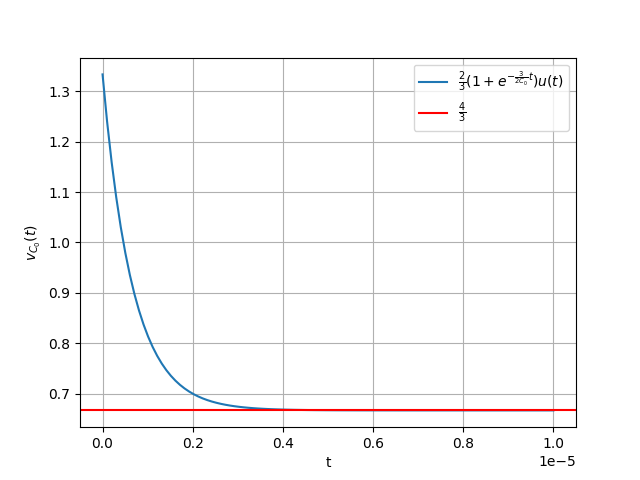
\includegraphics[width=\columnwidth]{./ques_3/3.4.png}
	\caption{$v_{C_0}(t)$ wrt t}	
	\label{fig:3.4}
\end{figure}
	\item Verify your result using ngspice.
\solution Run the below ngspice code to get data and then use given python file to plot fig. \ref{fig:3.5}
		In fig. \ref{fig:3.5}, we can see that both results are coinciding. So, our answer is correct
\begin{lstlisting}
https://github.com/himanshukumargupta11012/EE3900_assignments/blob/main/cktsig/ques_3/3.5.cir
https://github.com/himanshukumargupta11012/EE3900_assignments/blob/main/cktsig/ques_3/3.5.py
		\end{lstlisting}
\begin{figure}[!ht]
\centering
	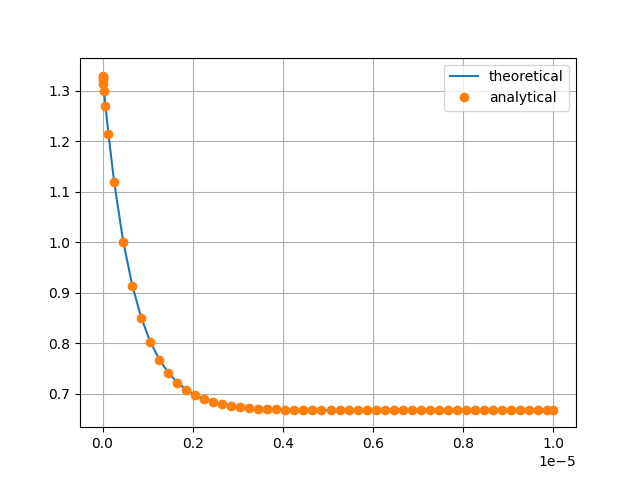
\includegraphics[width=\columnwidth]{./ques_3/3.5.png}
	\caption{theoretical v/s analytical}	
	\label{fig:3.5}
\end{figure}
	\item Find $v_{C_0}(0-), v_{C_0}(0+)$ and  $v_{C_0}(\infty) $. 
		\solution 
		Charge not changes abruptly.So,
		\begin{align}
			v_{C}(0^-)=v_{C}(0^+)&=v_{C}(0)\\
			&=\frac{2}{3}\brak{1+e^{-\frac{3\times 10^{6}\times 0}{2}}}u(0)\\
			&=\frac{4}{3}
		\end{align}
		and
		\begin{align}
			v_C(\infty)&=\lim_{t\to \infty}\frac{2}{3}\brak{1+e^{-\frac{3\times 10^{6}t}{2}}}u(t)\\
			&=\frac{2}{3}
		\end{align}
	\item Obtain the Fig.  in problem 
		\ref{prob:init}
			using the equivalent differential equation.
			\solution Using KCL at the junction of resistors and capacitor after joining S to Q in fig. \ref{crct:2.2}, we get
			\begin{align}
				\frac{v_{C}(t)-0}{R_1}+\frac{v_{C}(t)-v_{2}(t)}{R_2}+\frac{dq(t)}{dt}=0\\
			\end{align}
where $q(t)$ is charge on capacitor
Taking laplace both sides, we get
\begin{align}
	\frac{V_{C}(s)-0}{R_1}+\frac{V_{C}(s)-V_{2}(s)}{R_2}+sQ(s)-q(0)=0\\
	\frac{V_{C}(s)-0}{R_1}+\frac{V_{C}(s)-V_{2}(s)}{R_2}+sC_0\frac{Q(s)}{C_0}-q(0)=0\\
	\frac{V_{C}(s)-0}{R_1}+\frac{V_{C}(s)-V_{2}(s)}{R_2}+sC_0V_{C}-\frac{4}{3}C_0=0\\
	\frac{V_{C}(s)-0}{R_1}+\frac{V_{C}(s)-V_{2}(s)}{R_2}+\frac{V_{C}(s)-\frac{4}{3s}}{\frac{1}{sC_0}}=0\\
\end{align}
The above equation is same as equation of Fig. in problem 
		\ref{prob:init}
	\end{enumerate}
 \section{Bilinear Transform}
\begin{enumerate}[label=\arabic*.,ref=\thesection.\theenumi]
\numberwithin{equation}{section}
\item In Fig. 
			\ref{fig:ckt},
			consider the case when $S$ is switched to $Q$ right in the beginning. Formulate the differential equation.

			\solution 
			Applyling KCL after switching S to Q, we get differential equation
		\begin{align}
			\frac{v_{C_0}(t)-0}{R_1}+\frac{v_{C_0}(t)-v_2(t)}{R_2}+\frac{dq(t)}{dt}=0 \label{eq:4.1}\\
			\frac{v_{C_0}(t)-0}{R_1}+\frac{v_{C_0}(t)-v_2(t)}{R_2}+C_0\frac{d\cbrak{v_{C_0}(t)}}{dt}=0 \label{eq:4.1.2}
		\end{align}
		
		\item 		Find $H(s)$ considering the ouput voltage at the capacitor.

			\solution
			Taking laplace of eqn \eqref{eq:4.1}, we get
			\begin{align}		
				\frac{V_{C_0}(s)-0}{R_1}+\frac{V_{C_0}(s)-V_2(s)}{R_2}+&sQ(s)-q(0)=0\\
				\frac{V_{C_0}(s)-0}{R_1}+\frac{V_{C_0}(s)-V_2(s)}{R_2}+&sC_0V_{C_0}(s)=0\\
				\implies \frac{V_{C_0}(s)}{V_2(s)}=\frac{\frac{1}{R_2}}{\frac{1}{R_1}+\frac{1}{R_2}+sC_0}&\label{eq:4.2}\\
				\implies H(s)=\frac{\frac{1}{R_2}}{\frac{1}{R_1}+\frac{1}{R_2}+sC_0}\quad &\because H(s)=\frac{O}{I}
			\end{align}
Since at starting, capacitor is uncharged so $q(0)=0$ in above equation.

			We know that 
			\begin{align}
				H(s)&=\frac{\text{output}}
{\text{input}}\\
				&=\frac{V_{C_0}(s)}{V_2(s)}\\
				&=\frac{\frac{1}{R_2}}{\frac{1}{R_1}+\frac{1}{R_2}+sC_0}\label{eq:4.2.1}\quad \text{from \eqref{eq:4.2}}
			\end{align}
		\item Plot $H(s)$.  What kind of filter is it?
			
			\solution Run the following code to get fig \ref{fig:4.3}
			\begin{lstlisting}
https://github.com/himanshukumargupta11012/EE3900_assignments/blob/main/cktsig/ques_4/4.3.py
		\end{lstlisting}
		\begin{figure}
		\centering
		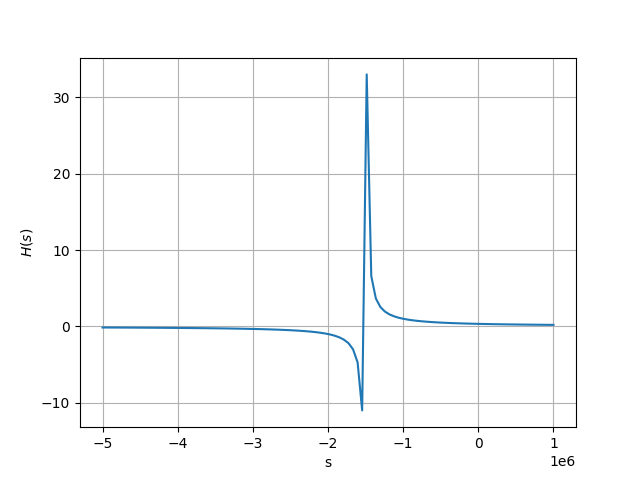
\includegraphics[width=\columnwidth]{./ques_4/4.3.png}
			\caption{$H(s)$ wrt s}	
		\label{fig:4.3}
\end{figure}
		As $\omega$ increases, s increases since $s=j\omega$. And as s increases H(s) decreases as we can see from fig. \ref{fig:4.3} or equation \eqref{eq:4.2.1}.

		So, conclusively as $\omega$ increses, $H(s)$ decreases. As high frequency passes from this it becomes negligible which is equivalent to removing high frequency. Hence, it is low-pass filter.

		\item Using trapezoidal rule for integration, formulate the difference equation
			by considering 
		\begin{align}
			y(n) = y(t)\vert_{t=n}
		\end{align}

		\solution
		From equation \eqref{eq:4.1.2}
		\begin{align}
\frac{v_{C_0}(t)-0}{R_1}+\frac{v_{C_0}(t)-v_2(t)}{R_2}+C_0\frac{d\cbrak{v_{C_0}(t)}}{dt}=0\\
\implies \frac{d\cbrak{v_{C_0}(t)}}{dt}=\frac{2u(t)-v_{C_0}(t)}{R_2C_0}-\frac{v_{C_0}(t)}{R_1C_0}
\\
			v_{C_0}(t)\bigg]_n^{n+1}=\int_n^{n+1}\brak{\frac{2u(t)-v_{C_0}(t)}{R_2C_0}-\frac{v_{C_0}(t)}{R_1C_0}}dt \label{eq:4.4.1}
		\end{align}
		From trapezoidal rule of integration
		\begin{align}
			\int_a^b f(x)dx=\brak{b-a}\frac{f(b)-f(a)}{2}
			\label{eq:trap_rule}
		\end{align}
	Using this rule in RHS of equation \eqref{eq:4.4.1}, we get
	\begin{align}
		v_{C_0}(n+1)-v_{C_0}(n)&=\frac{u(N+1+u(n)}{R_2C_0}\\
		&-\brak{\frac{1}{R_1}+\frac{1}{R_2}}\frac{v_{C_0}(n+1)+v_{C_0}(n)}{2C_0}
	\end{align}
	Since $v_{C_0}$ is output so $y(n)=v_{C_0}(n)$.

	So, difference equation will be
	\begin{align}
		&y(n+1)\brak{1+\frac{1}{2R_1C_0}+\frac{1}{2R_2C_0}}=\\
		&y(n)\brak{1-\frac{1}{2R_1C_0}-\frac{1}{2R_2C_0}}+\frac{u(n+1)+u(n)}{R_2C_0}
\end{align}
	\item Find $H(z)$.

		\solution
		Taking z-transform of difference equation we get,
		\begin{align}
			&zY(z)\brak{1+\frac{1}{2R_1C_0}+\frac{1}{2R_2C_0}}\\
			&=Y(z)\brak{1-\frac{1}{2R_1C_0}-\frac{1}{2R_2C_0}}+U(z)\frac{z+1}{R_2C_0}\\
			&\implies Y(z)\brak{z+\frac{z}{2R_1C_0}+\frac{z}{2R_2C_0}-1+\frac{1}{2R_1C_0}+\frac{1}{2R_2C_0}}\\
			&\quad \quad	=U(z)\frac{z+1}{R_2C_0}\\
			&\implies \frac{Y(z)}{2U(z)}=\frac{\frac{z+1}{2R_2C_0}}{\brak{z\brak{1+\frac{1}{2R_1C_0}+\frac{1}{2R_2C_0}}-1+\frac{1}{2R_1C_0}+\frac{1}{2R_2C_0}}}\\
			&\implies H(z)=\frac{\frac{z+1}{2R_2C_0}}{\brak{z\brak{1+\frac{1}{2R_1C_0}+\frac{1}{2R_2C_0}}-1+\frac{1}{2R_1C_0}+\frac{1}{2R_2C_0}}}\\
			&\quad \because H(s)=\frac{O}{I}
		\end{align}
	\item How can you obtain $H(z)$ from $H(s)$?
		
		\solution The z-transfrom can be obtained from laplace by substituting
		\begin{align}
			s=\frac{2}{L}\frac{1-z^{-1}}{1+z^{-1}}
		\end{align}
		where T is sampling time period or in simple words length of interval taken in trapezoidal equation. In our case $T=(n+1)-n=1$

		Putting this in equation \eqref{eq:4.2.1}, we get
		\begin{align}
			H(z)&=\frac{\frac{1}{R_2}}{\frac{1}{R_1}+\frac{1}{R_2}+2\frac{1-z^{-1}}{1+z^{-1}}C_0}\\
			&=\frac{\frac{z+1}{2R_2C_0}}{\brak{z\brak{1+\frac{1}{2R_1C_0}+\frac{1}{2R_2C_0}}-1+\frac{1}{2R_1C_0}+\frac{1}{2R_2C_0}}}
		\end{align}


\item Find $y(n)$ from $H(z)$ and verify whether $y(n) = y(t)\vert_{t = n}$.\\
	 \solution 
	 \begin{align}
		 &Y(z) = H(z)X(z) \\
		      &= \frac{2.5 \times 10^5\brak{1 + z^{-1}}}{z^{-1}\brak{7.5 \times10^5 -1} + 7.5\times 10^5 + 1}\frac{2}{1 - z^{-1}} \\
		      &= \frac{2}{3}\sbrak{\frac{1}{1-z^{-1}} - \frac{2}{3} \frac{1}{\brak{7.5 \times 10^5 - 1}z^{-1} + \brak{7.5 \times 10^5 +1}}}
	 \end{align}
	 Now if we apply inverse z-transform by taking ROC $\abs{z} > 1$,
	  \begin{align}
		  y(n) &= \frac{2}{3}u(n) - \frac{2}{3}\brak{-\frac{7.5 \times 10^5 -1}{7.5 \times 10^5 + 1}}^nu(n)
	  \end{align}
	  Here we used the following properties of z-transform,
	   \begin{align}
		   u(n) \ztrans \frac{1}{1-z^{-1}} , \abs{z} > 1\\
		   a^{n}u(n) \ztrans \frac{1}{1 - az^{-1}} ,\abs{z} >\abs{a}
	   \end{align}
	   Here we are sampling the signal at high frequency means at small intervals of time let say for $n = 0.5 \times 10^{-5} , 1 \times 10^{-5} \cdots$,for that we can approximate $y(n)$ as,
	    \begin{align}
		    y(n) \approx \frac{2}{3}\brak{ 1 - \frac{1 - 7.5 \times 10^5n}{1 + 7.5\times 10^5n}}u(n)
	    \end{align}
            Now we will verify it from $y(t)$, for that consider
	     \begin{align}
		     Y(s) &= H(s)X(s) \\
			  &=\frac{5 \times 10^5}{s + 1.5 \times 10^6}\frac{2}{s} \\
			  &= \frac{2}{3}\brak{\frac{1}{s} - \frac{1}{s + 1.5 \times 10^6}}
	     \end{align}
	     Now we will apply inverse laplace transform with ROC being $\mathcal{R}\cbrak{s} > 0$ on b.s,
	      \begin{align}
	           y(t) &= \frac{2}{3}\brak{1 - e^{-1.5\times 10^6t}}u(t)
              \end{align}
               Now 
	        \begin{align}
			e^{-1.5 \times 10^6t} &= \frac{e^{-7.5 \times 10^5t}}{e^{7.5 \times 10^5t}} \\
			&\approx \frac{1 - 7.5\times10^5t}{1 + 7.5\times10^5t} , \text{when}\, t << 10^{-6}
		\end{align}
	Using that,
	     \begin{align}
		     y(t) &= \frac{2}{3}\brak{1 - \frac{1 - 7.5\times10^5t}{1 + 7.5\times10^5t}}u(t)
	     \end{align}
	     And 
	      \begin{align}
		      y(t)\vert_{t = n} &= \frac{2}{3}\brak{1 - \frac{1 - 7.5\times10^5n}{1 + 7.5\times10^5n}}u(n)
              \end{align}
          As you can see both are turn to be the same.\\
	  Download the following codes for the simulation and plot \ref{fig:y_m} 
	   \begin{lstlisting}
wget https://github.com/himanshukumargupta11012/EE3900_assignments/blob/main/cktsig/ques_4/4.7.py
wget  https://github.com/himanshukumargupta11012/EE3900_assignments/blob/main/cktsig/ques_4/4.7.cir
           \end{lstlisting}
	   Then run the following command,
	\begin{lstlisting}
ngspice 4.7.cir
python3 4.7.py
        \end{lstlisting}
        \begin{figure}[!ht]
		\centering
		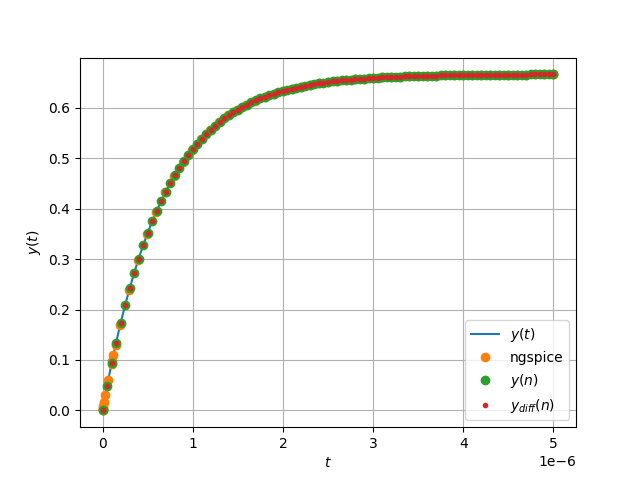
\includegraphics[width = \columnwidth]{./ques_4/4.7.png}
		\label{fig:y_m}
		\caption{Output of the filter vs time}		
        \end{figure}
	\end{enumerate}
\end{document}

